\documentclass[../../../../main.tex]{subfiles}
\begin{document}

\begin{flushright}
\footnotesize\textit{【自動文字起こし・要確認】}
\end{flushright}

\noindent
[\textbf{解}] $P$ が $ABCD$ を1周する時、
\[
\begin{cases}
AB \text{上} \dots y = 1, -1 \le x \le 1 & \dots \text{①} \\
BC \text{上} \dots x = -1, -1 \le y \le 1 & \dots \text{②} \\
CD \text{上} \dots y = -1, -1 \le x \le 1 & \dots \text{③} \\
DA \text{上} \dots x = 1, -1 \le y \le 1 & \dots \text{④}
\end{cases}
\]
である。従って、$Q(u, v)$ のキセキは以下。($a > 1$ に注意)

\begin{enumerate}
    \item[$1^\circ$] ①の時
    \[
    u = a \cdot a^x, \quad v = \frac{1}{a} \cdot a^{2x} \quad (-1 \le x \le 1)
    \]
    から、
    \[
    v = \frac{1}{a^3} u^2 \quad (1 \le u \le a^2)
    \]

    \item[$2^\circ$] ②の時
    \[
    u = \frac{1}{a} \cdot a^y, \quad v = \frac{1}{a^2} \cdot a^{-y} \quad (-1 \le y \le 1)
    \]
    から
    \[
    v = \frac{1}{a^3} \frac{1}{u} \quad \left(\frac{1}{a^2} \le u \le 1\right)
    \]

    \item[$3^\circ$] ③の時
    \[
    u = \frac{1}{a} \cdot a^x, \quad v = a \cdot a^{2x} \quad (-1 \le x \le 1)
    \]
    から
    \[
    v = a^3 u^2 \quad \left(\frac{1}{a^2} \le u \le 1\right)
    \]

    \item[$4^\circ$] ④の時
    \[
    u = a \cdot a^y, \quad v = a^2 \cdot a^{-y} \quad (-1 \le y \le 1)
    \]
    から
    \[
    v = a^3 \frac{1}{u} \quad (1 \le u \le a^2)
    \]
\end{enumerate}

図示して右図のようになる。求める面積 $S$ のうち $\frac{1}{a^2} \le u \le 1$ のものを $S_1$, $1 \le u \le a^2$ のものを $S_2$ として、
\[
S = S_1 + S_2 \quad \dots \text{⑤}
\]

\begin{center}
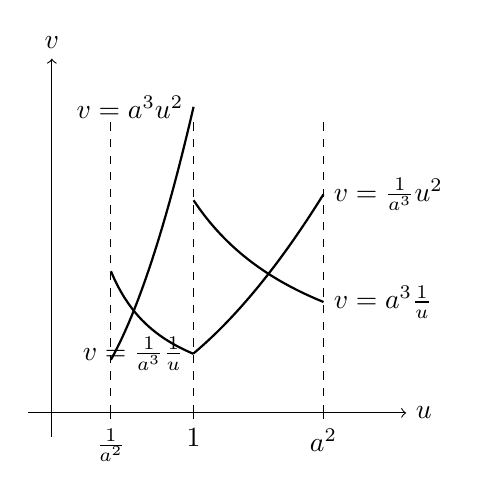
\begin{tikzpicture}[scale=1.5]
    \draw[->] (-0.2,0) -- (3,0) node[right]{$u$};
    \draw[->] (0,-0.2) -- (0,3) node[above]{$v$};
    \draw (0.5,0.05) -- (0.5,-0.05) node[below]{$\frac{1}{a^2}$};
    \draw (1.2,0.05) -- (1.2,-0.05) node[below]{$1$};
    \draw (2.3,0.05) -- (2.3,-0.05) node[below]{$a^2$};
    
    \draw[thick, domain=0.5:1.2] plot ({\x}, {1.8*\x*\x}) node[left]{$v=a^3 u^2$};
    \draw[thick, domain=0.5:1.2] plot ({\x}, {0.6/\x}) node[left]{$v=\frac{1}{a^3}\frac{1}{u}$};
    \draw[thick, domain=1.2:2.3] plot ({\x}, {2.16/\x}) node[right]{$v=a^3\frac{1}{u}$};
    \draw[thick, domain=1.2:2.3] plot ({\x}, {0.35*\x*\x}) node[right]{$v=\frac{1}{a^3}u^2$};
    \draw[dashed] (0.5,0) -- (0.5,2.5);
    \draw[dashed] (1.2,0) -- (1.2,2.5);
    \draw[dashed] (2.3,0) -- (2.3,2.5);
\end{tikzpicture}
\end{center}

\begin{align*}
S_1 &= \int_{\frac{1}{a^2}}^1 \left( a^3 u^2 - \frac{1}{a^3 u} \right) du \\
&= \left[ \frac{a^3}{3} u^3 - \frac{1}{a^3} \log u \right]_{\frac{1}{a^2}}^1 \\
&= \frac{a^3}{3} - \left( \frac{1}{3a^3} + \frac{2}{a^3} \log a \right) \\
&= \frac{1}{3}a^3 - \frac{1}{3a^3} - \frac{2}{a^3}\log a \\[10pt]
S_2 &= \int_1^{a^2} \left( a^3 \frac{1}{u} - \frac{1}{a^3} u^2 \right) du \\
&= \left[ a^3 \log u - \frac{1}{3a^3} u^3 \right]_1^{a^2} \\
&= 2a^3 \log a - \frac{1}{3}a^3 + \frac{1}{3a^3}
\end{align*}
⑤へ代入して、
\[
S = 2\left(a^3 - \frac{1}{a^3}\right)\log a
\]

\newpage

\end{document}
